\documentclass[11pt]{article}
\usepackage{geometry}
\geometry{a4paper, margin=2cm}

\usepackage{fontspec}
\setmainfont{DejaVu Serif}
\setmonofont{DejaVu Sans Mono}

\usepackage{listings}
\usepackage{xcolor}
\usepackage{enumitem}
\usepackage{titlesec}
\usepackage{hyperref}
\usepackage[breakable,skins]{tcolorbox}
\usepackage{fancyhdr}
\usepackage{amssymb}
\usepackage{tikz}
\usetikzlibrary{arrows.meta,positioning,shapes.geometric}

% ---------- Colors ----------
\definecolor{codebg}{RGB}{245,245,245}
\definecolor{httpblue}{RGB}{20,60,110}
\definecolor{causeorange}{RGB}{180,80,0}

% ---------- Listings styles ----------
\lstdefinestyle{http}{
    backgroundcolor=\color{codebg},
    basicstyle=\ttfamily\small,
    frame=single,
    rulecolor=\color{gray},
    columns=fullflexible,
    breaklines=true,
    breakatwhitespace=false,
    showstringspaces=false
}

\lstdefinestyle{code}{
    backgroundcolor=\color{codebg},
    basicstyle=\ttfamily\small,
    frame=single,
    rulecolor=\color{gray},
    columns=fullflexible,
    breaklines=true,
    language=Python,
    keywordstyle=\color{httpblue}\bfseries,
    commentstyle=\color{gray}\itshape,
    stringstyle=\color{causeorange},
    showstringspaces=false
}

% ---------- Headings ----------
\titleformat{\section}{\Large\bfseries\color{httpblue}}{\thesection}{1em}{}
\titleformat{\subsection}{\large\bfseries}{\thesubsection}{1em}{}
\titleformat{\subsubsection}{\normalsize\bfseries\itshape}{\thesubsubsection}{1em}{}

\pagestyle{fancy}
\fancyhf{}
\lhead{Gobuster --- Content \& Host Discovery}
\rhead{\thepage}
\setlength{\headheight}{14pt}

% ---------- Custom boxes ----------
\newtcolorbox{causebox}{
    breakable, colback=orange!5, colframe=causeorange,
    title=How It Works (Mechanism \& Why It Succeeds)
}

\newtcolorbox{labbox}[1]{
    breakable, colback=blue!4, colframe=httpblue,
    title=#1
}

\begin{document}

% ================= TITLE PAGE =================
\title{\textbf{Gobuster}\\\large Content \& Virtual Host Discovery --- Web Application Penetration Testing Notes}
\author{Eyad Islam El-Taher}
\date{}
\maketitle
\tableofcontents
\newpage

% ================= 1. INTRODUCTION =================
\section{Introduction}

\begin{itemize}
    \item Gobuster is a high-performance, Go-based brute-forcing tool written by Christian Mehlmauer and OJ Reeves, used to discover content and hosts that are not linked anywhere and therefore invisible to normal browsing or crawling.
    \item It operates in distinct \textbf{modes}, each targeting a different discovery surface: \texttt{dir} (files/directories), \texttt{dns} (subdomains), \texttt{vhost} (virtual hosts sharing one IP), \texttt{fuzz} (generic keyword substitution), plus \texttt{s3}, \texttt{gcs} (cloud storage buckets) and \texttt{tftp}.
\end{itemize}

% ================= 2. TECHNICAL BACKGROUND =================
\section{Technical Background}

\subsection{HTTP Routing and the Host Header}
\begin{itemize}
    \item A single web server (one IP, one port) can serve multiple distinct sites. The server decides which site's content to return based on the \texttt{Host} header sent in the HTTP request, not the IP address dialed.
    \item This is called \textbf{name-based virtual hosting}. Apache implements it via \texttt{<VirtualHost>} blocks matched on \texttt{ServerName}/\texttt{ServerAlias}; Nginx via \texttt{server\_name} directives inside \texttt{server \{\}} blocks.
    \item If a hostname is never advertised through public DNS or links, the only way to discover it is to guess candidate hostnames and observe whether the server responds differently --- this is exactly what \texttt{vhost} mode automates.
\end{itemize}

\subsection{DNS Resolution and Subdomain Structure}
\begin{itemize}
    \item Subdomains (e.g. \texttt{staging.example.com}) are DNS records (typically \texttt{A}, \texttt{AAAA}, or \texttt{CNAME}) under a parent zone. They can exist and resolve publicly even if never linked from the main site.
    \item \texttt{dns} mode brute-forces subdomain names and performs a live DNS resolution for each candidate; a response means the record exists.
    \item \textbf{Wildcard DNS} is the main technical pitfall: some zones resolve \emph{any} subdomain (even nonsense ones) to a catch-all IP, which would otherwise flood results with false positives. Gobuster detects wildcards automatically and Gobuster's \texttt{--wildcard} flag forces the scan to continue anyway once detected.
\end{itemize}

\subsection{Content Discovery via Directory/File Brute-Forcing}
\begin{itemize}
    \item \texttt{dir} mode requests each wordlist entry as a path against the target and inspects the HTTP status code (and optionally response length) to decide if the resource exists.
    \item Frameworks frequently leave predictable artifacts reachable but unlinked: \texttt{/.git/HEAD}, \texttt{/backup.zip}, \texttt{/admin}, \texttt{/api/v1/}, \texttt{/.env} --- none of these appear in any menu, yet all are directly requestable.
\end{itemize}


% ================= 3. MODE ANATOMY =================
\section{Mode Anatomy}

\subsection{\texttt{dir} --- Directory/File Enumeration}
\begin{itemize}
    \item Iterates a wordlist over URL paths, classifies responses by status code (default positive set: \texttt{200,204,301,302,307,401,403}).
    \item Attack surface: any path-addressable resource --- backup files, config files, forgotten admin routes, API versioning paths (\texttt{/api/v2/}), source control artifacts.
\end{itemize}
\begin{causebox}
Servers do not enumerate their own file tree to visitors; a nonexistent path simply returns \texttt{404}, and an existing-but-unlinked path returns \texttt{200}/\texttt{301} identically to a linked one. There is no cryptographic or access-control difference between ``linked'' and ``unlinked'' content --- only obscurity. Any developer who ships \texttt{/backup.sql} into the webroot without an authentication check is trusting that nobody guesses the name; brute-forcing defeats that trust trivially.
\end{causebox}

\subsection{\texttt{dns} --- Subdomain Enumeration}
\begin{itemize}
    \item Brute-forces subdomain labels and resolves each against the authoritative or a specified resolver.
    \item Attack surface: any subdomain that exists as a DNS record, whether or not a certificate or working service sits behind it.
\end{itemize}
\begin{causebox}
DNS zones are queried, not crawled --- a client can ask ``does \texttt{X.example.com} exist?'' directly, and the resolver answers truthfully regardless of whether \texttt{X} is publicly advertised anywhere. Organizations that provision \texttt{staging.example.com} or \texttt{old-admin.example.com} in DNS for internal convenience, assuming ``nobody will find it because it isn't linked,'' are relying on the same false obscurity as unlinked \texttt{dir} content.
\end{causebox}

\subsection{\texttt{vhost} --- Virtual Host Enumeration}
\begin{itemize}
    \item Sends requests to a single IP/URL while iterating the \texttt{Host} header value, then compares response length/status/body to a baseline to detect a genuinely different site.
    \item Attack surface: any vhost configured server-side but never given a public DNS record --- e.g.\ an internal admin console reachable only if you already know its hostname.
\end{itemize}
\begin{causebox}
Name-based virtual hosting means the web server, not DNS, holds the authoritative list of what hostnames it will serve. A request can reach the correct \emph{virtual host block} purely by carrying the right \texttt{Host} header, even if that hostname resolves nowhere in public DNS or resolves only to a different IP entirely. Admins who assume ``this vhost is safe because it isn't in DNS'' are wrong: DNS and vhost configuration are two independent, decoupled mechanisms.
\end{causebox}

\subsection{\texttt{fuzz} --- Generic FUZZ Substitution}
\begin{itemize}
    \item Replaces a literal \texttt{FUZZ} marker anywhere in the URL, headers, or POST body with wordlist entries. Not restricted to a fixed position like \texttt{dir}/\texttt{vhost}.
    \item Attack surface: GET/POST parameter values, custom headers, arbitrary body fields --- anywhere user-controlled input might reach a sensitive sink (SSRF-prone \texttt{format=} or \texttt{url=} parameters, IDOR-prone numeric IDs, auth-bypass headers).
\end{itemize}
\begin{causebox}
Because the position of the payload is entirely user-defined via the \texttt{FUZZ} token, this mode has no assumption about \emph{where} untrusted input matters --- it mirrors the general principle that any attacker-influenced value (not just the URL path) can be a discovery/attack vector if the backend logic branches on it (e.g.\ a \texttt{format} parameter selecting a code path that fetches a URL server-side).
\end{causebox}

% ================= 4. PRACTICAL USAGE & FLAGS =================
\section{Practical Usage \& Flags}

\subsection{\texttt{dir} Mode --- Basic to Advanced}

Basic sweep with a common wordlist:
\begin{lstlisting}[style=http]
gobuster dir -u https://target.com -w /usr/share/wordlists/dirb/common.txt
\end{lstlisting}

Add extensions and filter noise by status code:
\begin{lstlisting}[style=http]
gobuster dir -u https://target.com \
  -w /usr/share/wordlists/SecLists/Discovery/Web-Content/raft-large-words.txt \
  -x php,bak,old,zip,tar.gz,env \
  -s 200,204,301,302,307,401,403 -t 50
\end{lstlisting}

Authenticated brute-force behind a session cookie, following redirects, ignoring TLS errors:
\begin{lstlisting}[style=http]
gobuster dir -u https://target.com/account \
  -w raft-large-words.txt \
  -c "session=<SESSION>" -r -k -o results.txt
\end{lstlisting}

Advanced: hide soft-404 pages that all return \texttt{200} with identical body length:
\begin{lstlisting}[style=http]
gobuster dir -u https://target.com -w common.txt --exclude-length 9265
\end{lstlisting}

\subsection{\texttt{dns} Mode --- Basic to Advanced}

Basic subdomain sweep:
\begin{lstlisting}[style=http]
gobuster dns -d target.com \
  -w SecLists/Discovery/DNS/subdomains-top1million-5000.txt -t 50
\end{lstlisting}

Advanced: reveal CNAMEs (useful for spotting dangling-CNAME subdomain-takeover candidates), force through a wildcard zone, use a specific resolver to dodge local rate limiting:
\begin{lstlisting}[style=http]
gobuster dns -d target.com -w subdomains-top1million-20000.txt \
  -r 1.1.1.1 -c --wildcard -t 100
\end{lstlisting}

\subsection{\texttt{vhost} Mode --- Basic to Advanced}

Basic vhost sweep against a known IP, appending the base domain to each wordlist entry:
\begin{lstlisting}[style=http]
gobuster vhost -u http://10.10.10.5 -w subdomains.txt --append-domain
\end{lstlisting}

Advanced: skip TLS verification, output results, then manually confirm a genuine hit by diffing response length against the baseline (vhost mode lacks \texttt{-s}/\texttt{-b} status-code filters, so false positives from catch-all vhosts are common and must be checked by hand):
\begin{lstlisting}[style=http]
gobuster vhost -u https://10.10.10.5 -w subdomains-top1million-20000.txt \
  --append-domain -k -o vhost_results.txt
\end{lstlisting}

Realistic raw request that gobuster is effectively automating, and the request you would replay manually in Burp Repeater once a candidate hit is found:
\begin{lstlisting}[style=http]
GET / HTTP/1.1
Host: intranet.target.com
Cookie: session=<SESSION>
User-Agent: Mozilla/5.0
Connection: close

HTTP/1.1 200 OK
Content-Type: text/html
Content-Length: 4821
Set-Cookie: PHPSESSID=<REDACTED>; path=/
\end{lstlisting}

\subsection{\texttt{fuzz} Mode --- Basic to Advanced}

Parameter value fuzzing:
\begin{lstlisting}[style=http]
gobuster fuzz -u "https://target.com/export?format=FUZZ" \
  -w format_payloads.txt -b 404
\end{lstlisting}

POST body fuzzing (e.g.\ probing an IDOR-prone identifier):
\begin{lstlisting}[style=http]
gobuster fuzz -u https://target.com/api/invoice \
  -m POST -d "invoice_id=FUZZ" \
  -H "Content-Type: application/x-www-form-urlencoded" \
  -H "Cookie: session=<SESSION>" -b 403
\end{lstlisting}

Custom header fuzzing (testing for header-based access-control bypass):
\begin{lstlisting}[style=http]
gobuster fuzz -u https://target.com/admin \
  -H "X-Forwarded-For: FUZZ" -w bypass_ips.txt
\end{lstlisting}

Realistic HTTP request rendered from the above (auth-bypass attempt via trusted-header spoofing):
\begin{lstlisting}[style=http]
GET /admin HTTP/1.1
Host: target.com
X-Forwarded-For: 127.0.0.1
Cookie: session=<SESSION>
Connection: close

HTTP/1.1 200 OK
Content-Length: 6120
\end{lstlisting}

\begin{center}
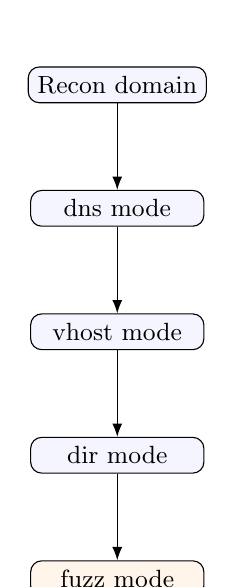
\begin{tikzpicture}[node distance=1.1cm, every node/.style={font=\small}]
    \node[draw, rounded corners, fill=blue!4, minimum width=2.2cm] (n1) {Recon domain};
    \node[draw, rounded corners, fill=blue!4, minimum width=2.2cm, below=of n1] (n2) {dns mode};
    \node[draw, rounded corners, fill=blue!4, minimum width=2.2cm, below=of n2] (n3) {vhost mode};
    \node[draw, rounded corners, fill=blue!4, minimum width=2.2cm, below=of n3] (n4) {dir mode};
    \node[draw, rounded corners, fill=orange!8, minimum width=2.2cm, below=of n4] (n5) {fuzz mode};
    \draw[-Latex] (n1) -- (n2);
    \draw[-Latex] (n2) -- (n3);
    \draw[-Latex] (n3) -- (n4);
    \draw[-Latex] (n4) -- (n5);
\end{tikzpicture}
\end{center}
\begin{center}
\small\textit{Figure 2: Typical discovery escalation order --- widen the attack surface (dns, vhost) before drilling into content (dir) and finally parameter-level logic (fuzz).}
\end{center}

% ================= 5. TOOLS & METHODOLOGY =================
\section{Tools \& Methodology}

\begin{itemize}
    \item \textbf{SecLists} --- the standard wordlist repository (\texttt{Discovery/Web-Content} for \texttt{dir}, \texttt{Discovery/DNS} for \texttt{dns}/\texttt{vhost}).
    \item \textbf{Burp Suite} --- send confirmed hits to Repeater for manual follow-up; Burp's built-in Content Discovery / Intruder can cross-validate gobuster findings.
    \item \textbf{subfinder} / \textbf{amass} --- passive subdomain enumeration (certificate transparency logs, search engines) to seed or supplement gobuster's active \texttt{dns} brute-force.
    \item \textbf{httpx} --- mass HTTP probing of resolved subdomains/vhosts to quickly triage which are alive and worth deeper inspection.
    \item \textbf{ffuf} --- a common alternative/companion to \texttt{fuzz} mode with more flexible multi-wordlist and recursive fuzzing.
\end{itemize}

Methodology (map $\rightarrow$ identify $\rightarrow$ confirm $\rightarrow$ escalate), adapted to discovery work:
\begin{enumerate}
    \item \textbf{Step 1 --- Passive recon.} Gather known subdomains via \texttt{subfinder}/certificate transparency before touching the target directly.
    \item \textbf{Step 2 --- Active DNS sweep.} Run \texttt{dns} mode to catch anything passive sources missed; note wildcard behavior early.
    \item \textbf{Step 3 --- VHost sweep.} Once IPs are known, run \texttt{vhost} mode against each IP to surface hosts with no public DNS record at all.
    \item \textbf{Step 4 --- Content discovery.} Run \texttt{dir} mode against every live host found, using a stack-appropriate wordlist once the technology is fingerprinted.
    \item \textbf{Step 5 --- Parameter/logic fuzzing.} Use \texttt{fuzz} mode on interesting endpoints found in Step 4 to probe parameter values, headers, and body fields.
\end{enumerate}

\textbf{Mindset:} treat every ``clean'' site as incomplete until content discovery has run. Common tells that discovery will pay off: a site with a CMS (predictable admin paths), recently migrated infrastructure (stale staging vhosts), or an API with visible versioning (\texttt{/v1/} implies \texttt{/v2/} may also exist). Common misconception: a \texttt{404} for the root path does not mean the host has no hidden content --- it only means that one path is unmapped.

\subsection{Checklist}
\begin{itemize}[label=$\square$]
    \item Confirm scope/authorization before any brute-force traffic is sent.
    \item Run passive subdomain recon before active \texttt{dns} brute-force.
    \item Check for wildcard DNS before trusting \texttt{dns} mode results.
    \item Run \texttt{vhost} mode against every known IP, not just the primary hostname.
    \item Cross-check \texttt{vhost} hits by comparing response length/body, not status code alone.
    \item Tune \texttt{dir} wordlist and extensions to the fingerprinted stack (CMS, framework).
    \item Set sane thread counts (\texttt{-t}) to avoid unintentional denial-of-service or IDS/WAF bans.
    \item Fuzz interesting parameters/headers found during content discovery with \texttt{fuzz} mode.
    \item Log all output (\texttt{-o}) for reporting and later diffing between engagement phases.
\end{itemize}


% ================= 9. BYPASSES & EDGE CASES =================
\section{Bypasses \& Edge Cases}

\begin{itemize}
    \item \textbf{Wildcard DNS false positives.} A zone that resolves any subdomain to a catch-all IP will make every \texttt{dns}-mode guess look like a hit unless \texttt{--wildcard} handling and manual verification are used.
    \item \textbf{Vhost catch-all false positives.} Servers without a proper default vhost return the same page for every Host header tried, inflating apparent hits --- always diff response length/body against a known-bad control hostname.
    \item \textbf{Case sensitivity.} Some servers/filesystems are case-sensitive (Linux) while others are not (Windows/IIS); running a wordlist with mixed casing variants can surface additional hits on case-sensitive targets.
    \item \textbf{Rate-limit evasion vs.\ noise trade-off.} Lower thread counts (\texttt{-t}) and added \texttt{--delay} reduce detection risk but slow discovery; aggressive threading risks WAF bans or denial-of-service on fragile targets.
    \item \textbf{Forgetting extensions.} \texttt{dir} mode does not append extensions by default --- \texttt{/config} will be found but \texttt{/config.php} will not unless \texttt{-x php} is set explicitly.
    \item \textbf{No recursion.} Gobuster does not recurse into discovered directories automatically; a fresh \texttt{dir} run must be issued against each newly found directory.
\end{itemize}


% ================= APPENDICES =================
\newpage
\section*{Appendices}
\addcontentsline{toc}{section}{Appendices}

\subsection*{A. Cheatsheet}
\begin{center}
\small
\begin{tabular}{|l|l|p{7.5cm}|}
\hline
\textbf{Mode} & \textbf{Flag} & \textbf{Effect} \\
\hline
dir & \texttt{-u} & Target URL \\
dir & \texttt{-w} & Wordlist \\
dir & \texttt{-x} & Extensions to append (\texttt{php,bak,zip}) \\
dir & \texttt{-s} / \texttt{-b} & Status codes to show / blacklist \\
dir & \texttt{-r} & Follow redirects \\
dir & \texttt{-k} & Skip TLS certificate verification \\
dir & \texttt{-c} & Cookies for the requests \\
dir & \texttt{-H} & Custom header, e.g.\ \texttt{-H "Authorization: Bearer <TOKEN>"} \\
dir & \texttt{--exclude-length} & Hide responses of a given byte length (soft-404 filtering) \\
\hline
dns & \texttt{-d} & Target domain \\
dns & \texttt{-r} & Custom DNS resolver \\
dns & \texttt{-c} & Show CNAME records \\
dns & \texttt{-i} & Show resolved IPs \\
dns & \texttt{--wildcard} & Force continued operation when wildcard DNS is found \\
\hline
vhost & \texttt{-u} & Target URL/IP \\
vhost & \texttt{-w} & Vhost wordlist \\
vhost & \texttt{--append-domain} & Append base domain to each wordlist entry \\
vhost & \texttt{-k} & Skip TLS certificate verification \\
\hline
fuzz & \texttt{-u} & URL containing the \texttt{FUZZ} marker \\
fuzz & \texttt{-m} & HTTP method (e.g.\ \texttt{POST}) \\
fuzz & \texttt{-d} & POST body containing \texttt{FUZZ} \\
fuzz & \texttt{-H} & Header containing \texttt{FUZZ} \\
\hline
global & \texttt{-t} & Thread count \\
global & \texttt{-o} & Output file \\
global & \texttt{--delay} & Delay between requests per thread \\
\hline
\end{tabular}
\end{center}

\end{document}